\section{Technische Dokumentation}
\subsection{Dokumentation der Storys}
\subsection{Klassendiagramme}
\subsection{Sequenzdiagramme}
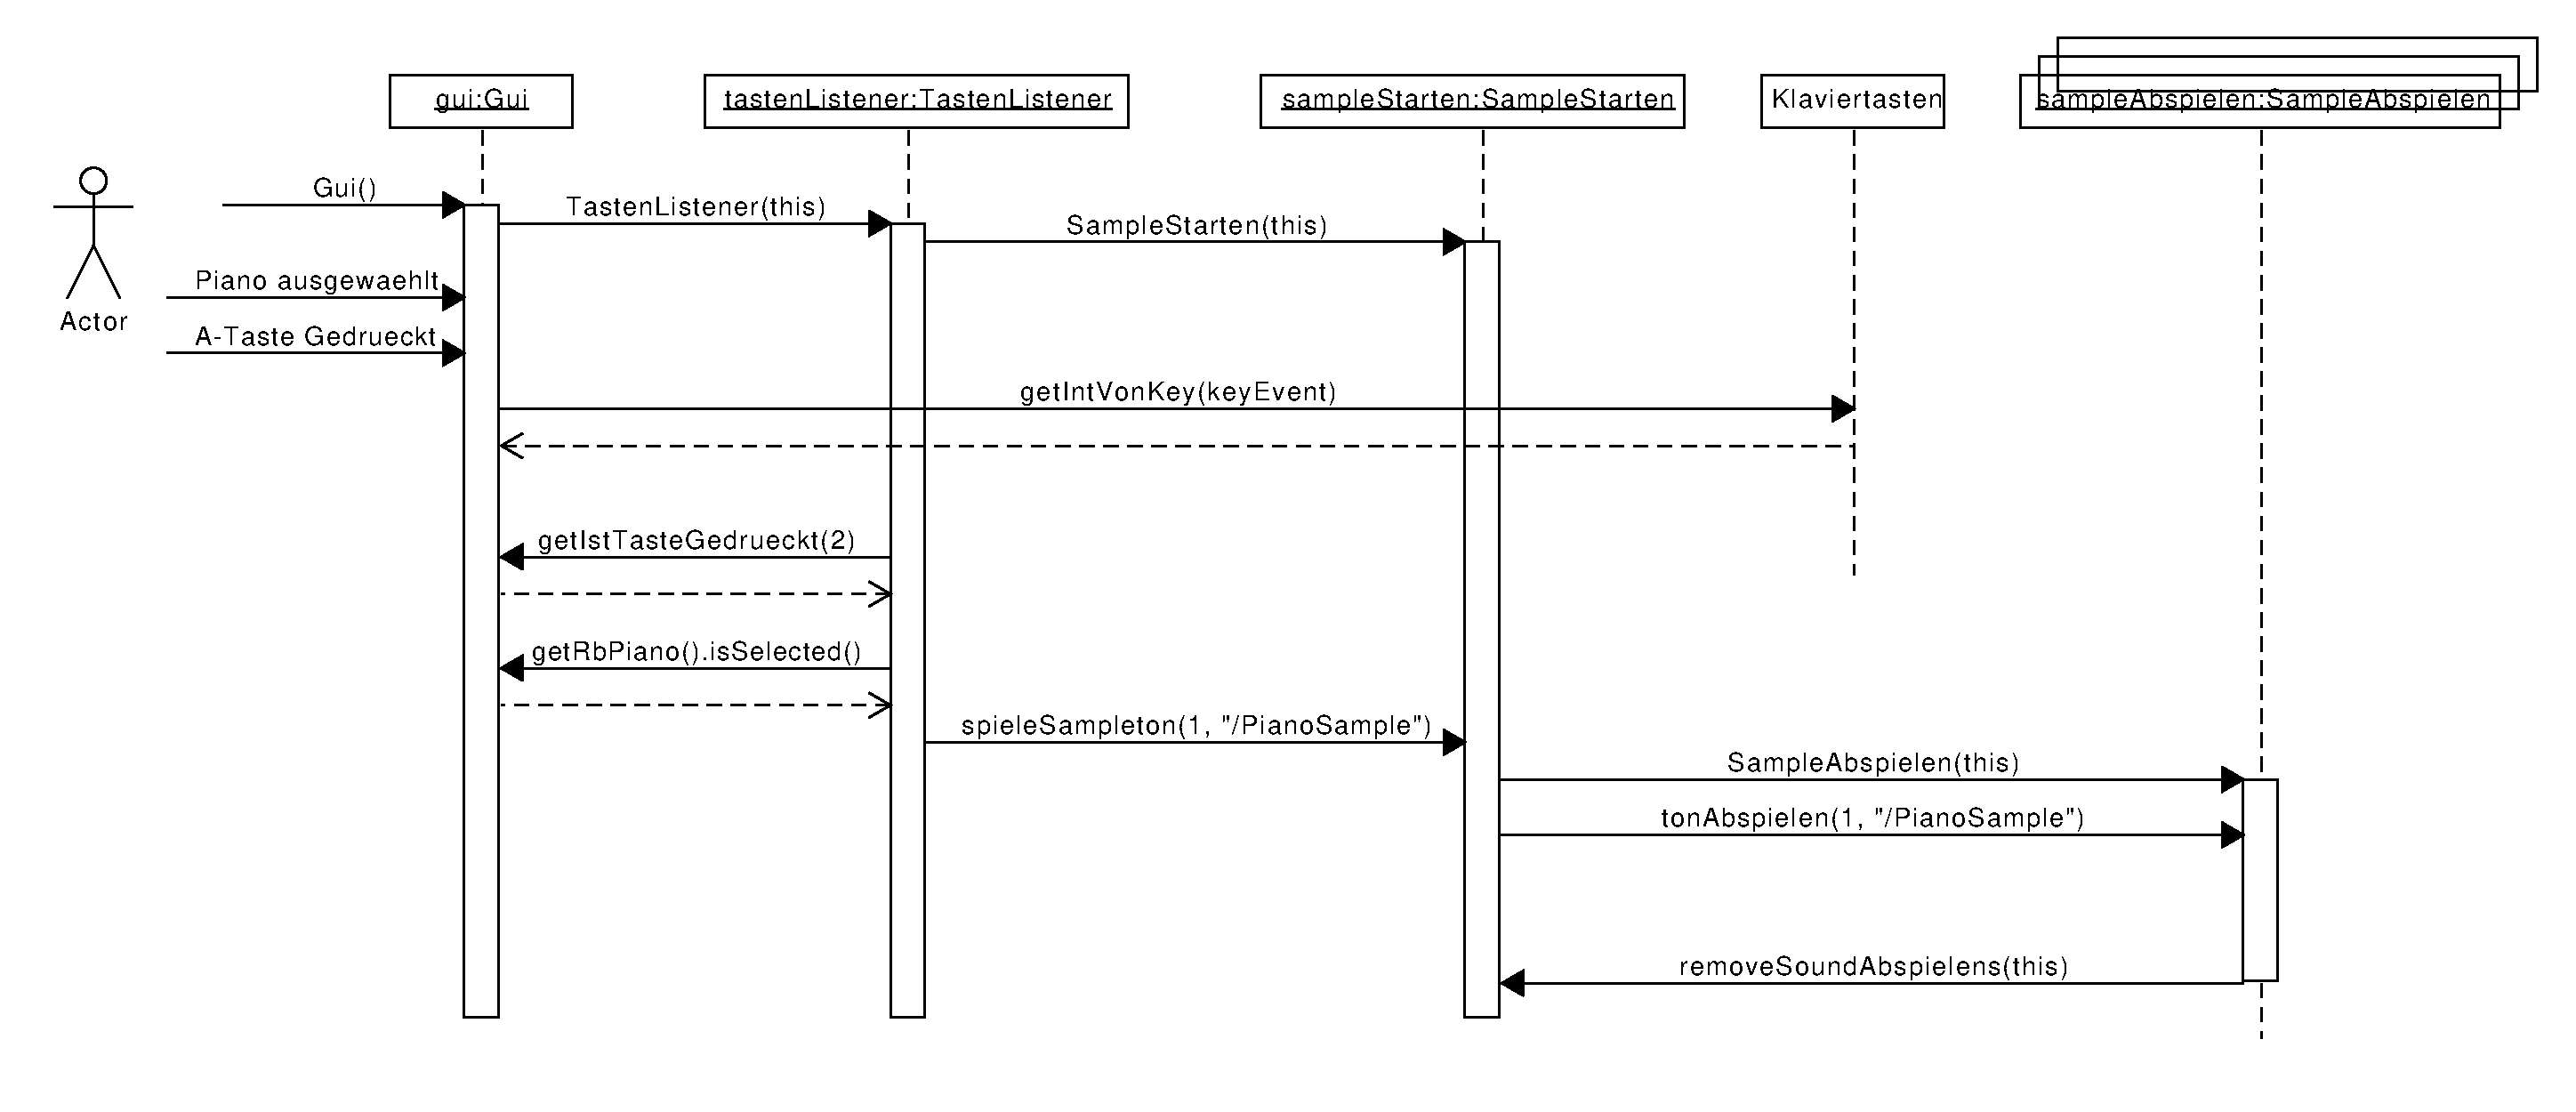
\includepdf{PDF/Klaviertaste_Gedrueckt.pdf}

\subsection{Beschreibung einiger Methoden}
Wir haben während des Projekts alle Methoden mithilfe von Javadocs dokumentiert. Unser komplettes 
Project ist also hier einsehbar: %Javadoc Zeug
\\

Einige größere Methoden werden wir in dieser Dokumentation allerdings etwas genauer beschreiben.

\subsection{Javadocs}
Der komplette Quelltext wurde mittels Javadocs auskommentiert. Hier kann nachgelesen werden, welche 
funktion die einzelnen Methoden erfüllen, sowie ihre Übergabe- und Rückgabeparameter, bzw. 
Exeptions  eingesehen werden.\\
Die komplette Javadocs Dokumentation kann hier geöffnet werden:\\
\url{./JavaDocs/index.html}